% ============================================================
% ============================================================

\documentclass[12pt, a4paper, oneside]{ctexart}

% ── 1. 数学与链接 ──
\usepackage{amsmath, amsthm, amssymb}
\usepackage[bookmarks=true, colorlinks, citecolor=blue, linkcolor=black]{hyperref}

% ── 2. 字体方案（newtxmath Times 风格） ──
\usepackage{newtxmath}

% ── 3. 页面布局（2.5cm 边距） ──
\usepackage[a4paper, margin=2.5cm, footskip=1cm]{geometry}

% ── 4. 页眉页脚 ──
\usepackage{fancyhdr}
\usepackage{lastpage}
\pagestyle{fancy}
\fancyhf{}
\fancyfoot[C]{数学试题第\thepage 页（共\pageref{LastPage}页）}
\renewcommand{\headrulewidth}{0pt}
\renewcommand{\footrulewidth}{0pt}

% ── 5. 表格与插图 ──
\usepackage{graphicx}
\usepackage{adjustbox}
\usepackage{booktabs}  % 三线表 \toprule/\midrule/\bottomrule，规则要求表格必须用它
\usepackage{array}
\usepackage{diagbox}
\usepackage{makecell}
\usepackage{caption}
\usepackage{float}
\usepackage{wrapfig}   % 图片场景2/4 依赖 wrapfigure，缺此包会 Undefined control sequence
\usepackage{tikz}

% ── 6. 选择题选项（tasks 环境） ──
\usepackage{tasks}
\settasks{
    label       = \Alph*.,
    label-width = 1.8em,
    item-indent = 2.4em,
    label-offset = 0.5em,
    column-sep  = 2em,
    before-skip = 0pt,
    after-skip  = 0pt
}

% ── 7. 大题编号（enumitem 体系，支持三级嵌套） ──
\usepackage[shortlabels]{enumitem}
\newlist{examenum}{enumerate}{3}
\setlist[examenum,1]{label=\arabic*., leftmargin=2em, itemsep=0.3em, parsep=0em}
\setlist[examenum,2]{label=(\arabic*), leftmargin=1.5em, itemsep=0.1em, parsep=0em}
\setlist[examenum,3]{label=(\roman*), leftmargin=1.5em, itemsep=0.1em, parsep=0em}

% ── 8. 自定义命令 ──
\newcommand{\mycircled}[1]{%
  \tikz[baseline=(char.base),outer sep=0pt]{%
    \node[draw,circle,inner sep=0.5pt,minimum size=1.4em,
          line width=0.4pt,font=\zihao{-5}] (char) {#1};%
  }%
}

\usepackage{newunicodechar}
\newunicodechar{①}{\mycircled{1}}
\newunicodechar{②}{\mycircled{2}}
\newunicodechar{③}{\mycircled{3}}
\newunicodechar{④}{\mycircled{4}}
\newunicodechar{⑤}{\mycircled{5}}
\newunicodechar{⑥}{\mycircled{6}}
\newunicodechar{⑦}{\mycircled{7}}
\newunicodechar{⑧}{\mycircled{8}}
\newunicodechar{⑨}{\mycircled{9}}
\newunicodechar{⑩}{\mycircled{10}}
\newcommand{\Parallel}{\raisebox{0.1ex}{\rotatebox[origin=c]{-20}{$\parallel$}}}
\newcommand{\bigstarraised}{\raisebox{0.2ex}{$\bigstar$}}
\newcommand{\blank}{\underline{\hspace{2cm}}}
\newcommand{\subjecttitle}[1]{{\fontsize{24pt}{22pt}\selectfont\centering\textbf{#1}\par}}
\newcommand{\subtitle}[1]{{\fontsize{16pt}{16pt}\selectfont\centering #1\par}}
\newcommand{\mi}{\mathrm{i}}
\newcommand{\me}{\mathrm{e}}

% ── 9. 答题空间（纯留白，无线条无边框）──
\newcommand{\answern}{%
  \par\vspace{3em}%
}

% ============================================================
% ============================================================

\graphicspath{{images/}}
\begin{document}

\begin{center}
    \LARGE{\textbf{2026 年测试卷（几何配图）}}
\end{center}

\vspace{0.5em}

\noindent\textbf{一、选择题：本题共1小题，每小题5分，共5分。}

\begin{enumerate}[itemsep=0.3em]
    \item 某几何体的三视图如图所示，则该几何体的体积为
    \begin{tasks}(4)
        \task $4$
        \task $6$
        \task $8$
        \task $12$
    \end{tasks}
\end{enumerate}

\noindent\textbf{四、解答题：本题共2小题，共24分。}

\begin{wrapfigure}{r}{0.30\textwidth}
\centering
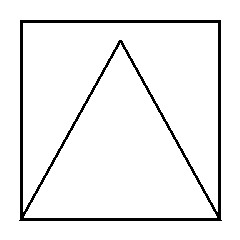
\includegraphics[width=\linewidth]{fig1.png}
\caption*{第2题图}
\end{wrapfigure}
\begin{examenum}[start=2, itemsep=1.5cm]
    \item （12分）如图，在四棱锥 $Q-ABCD$ 中，底面 $ABCD$ 是正方形，$QA \perp$ 平面 $ABCD$.
    \begin{examenum}
        \item 证明：$BQ \perp AD$；
        \item 若 $QB=\sqrt{6}$，求平面 $QAD$ 与平面 $QBC$ 夹角的余弦值.
    \end{examenum}
    \answern

    \item （12分）三个几何体的三视图分别如图①②③所示，求它们的表面积之和.
\end{examenum}

\begin{figure}[H]
\centering
\begin{minipage}[t]{0.28\textwidth}
\centering
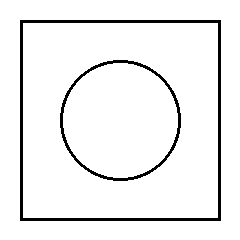
\includegraphics[width=\linewidth,height=2.5cm,keepaspectratio]{fig2.png}
\caption*{①}
\end{minipage}
\hfill
\begin{minipage}[t]{0.28\textwidth}
\centering
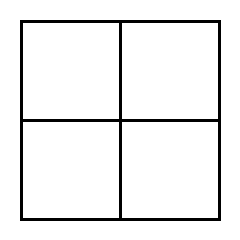
\includegraphics[width=\linewidth,height=2.5cm,keepaspectratio]{fig3.png}
\caption*{②}
\end{minipage}
\hfill
\begin{minipage}[t]{0.28\textwidth}
\centering
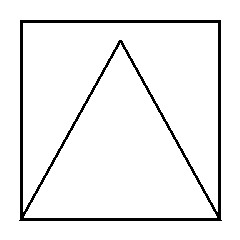
\includegraphics[width=\linewidth,height=2.5cm,keepaspectratio]{fig4.png}
\caption*{③}
\end{minipage}
\end{figure}

\end{document}
